The main action evidence begins with local scalar consequences, followed by controlled cue and historical-order assays that expose different informational requirements. The spatial process and regenerative experiments then test how acquired content affects actual bodily outcomes. Their hosts and continuations remain distinct.

\subsection*{Local paid consequences can establish an action direction without a supplied gradient}

Our primary action-learning test restricts the learner to consequences that its own moving material actually receives. A conservative, deformable cellular body starts with no learned response direction on a periodic $32\times32$ domain. Its local policies can read transported internal records, a locally completed scalar energy gain or loss, a receipt that motion was paid, and their own exploration randomness. The actual transport operator $K$ moves material and these records but supplies no displacement observation to the learner. Neither reward gradients, coordinates, the external field, the physical actuator rotation nor an environmental change flag enter the policy. This restriction separates the present capability from the gradient-following and motion-observing comparisons considered below (Fig.~\ref{fig:scalar-action}).

Movement axes, cohesion, pressure, energy transduction, exploration and material transport remain engineered capabilities. Two noise seeds are paired with opposite unknown actuator rotations, while the initial reward meaning is the same. These are two constructed conditions, not independent draws from a population of environments. Actual outcomes are available throughout a dense finite substrate. The task tests whether these local scalar experiences can establish useful action in an unfamiliar execution relationship; it does not test sparse encounter recovery, discovery of a sensor, or learning during tissue birth.

We compare standard accumulated action updates, the same updates with scalar state features, a fixed run-and-tumble response and a random policy. A subsequent prospectively fixed single-trajectory perturbation-response estimator maintains a moving estimate of the correlation between its action perturbation and the change in its actual scalar outcome over a completed eight-step action block. Its normalized estimate sets the next mean command. It receives no additional observation and has the same action bound and exploration schedule. The estimator and its normalized readout change together, so the comparison does not isolate an advantage of the estimator alone. The method is a standard local response rule, rather than a new optimizer or a measurement of the body's exact mechanical Jacobian.

Both response-estimation lives pass acquisition. Their final-64-step mass-weighted field scores are $0.63550$ and $0.63274$. After an unannounced reversal of reward meaning, the corresponding scores are $0.14684$ and $0.27984$: only the second condition passes the original complete phase criterion. In the subsequent 128 steps without new payments, outcome observations or parameter writes, both pass, with scores $0.53410$ and $0.60963$. These aftereffects do not repair the first condition's failed reversal. The first body's first continuous 32-step favourable interval occurs at step 678, after the reversal interval ended at 640; the second reaches that measure at 628. Neither result is recovery after a single new feedback event.

The strong comparisons constrain the interpretation. Both accumulated-action and scalar-context updates acquire in both conditions but pass neither reversal nor the aftereffect. Adding the tested state features therefore supplies no additional capability. Fixed run-and-tumble acquires in one condition and random action in neither; neither passes the later phases. The complete five-method, two-condition, three-phase results and all phase costs remain in Supplementary Tables~\ref{tab:scalar-phases} and \ref{tab:scalar-costs}. The response-estimation bodies finish at energies $121.308$ and $124.319$, spending $2.56720$ and $2.57260$ on movement. Fixed run-and-tumble spends less, $2.10862$ and $2.16194$, while finishing at $119.388$ and $119.294$. Useful acquired behaviour need not minimize movement expenditure, but the expenditure is part of its physical consequence.

\subsection*{Acquired direction contributes to an aftereffect without explaining every retained success}

We next branch each complete response-estimation body at step 640, including the body that failed its reversal window. Clearing its response estimate or rotating it by $90^\circ$ is followed by 128 actual steps without new feedback or writes. Original retained-content tails are reused as recorded references, not simulated again. Density, energy, other internal records, physical coupling, random state and clock agree at branching; the intervention changes only the declared response content. Rotation preserves each local estimate's norm, although the componentwise actuator nonlinearity means it need not preserve actual commands or costs.

Retained, cleared and rotated estimates produce aftereffect scores $0.53410/0.22435/0.14044$ in the first parent and $0.60963/0.34531/0.19537$ in the second. Both retained futures pass, one cleared future passes, and neither rotated future passes. Direction content therefore changes the physical future, while the acquired body's position and continued motion also contribute to occupancy. Clearing does not freeze the body: random commands, material transport and physical costs continue. The surviving cleared success rules out attributing every aftereffect to the retained direction. The two parents and their related futures are mechanism comparisons, not six independent acquisitions (Supplementary Table~\ref{tab:scalar-content}).

\subsection*{Execution changes require responsiveness, but a fixed response rule can suffice}

Changing reward meaning and changing the action--consequence relationship pose different problems. From the two actual response-estimation parents at step 320, we retain the original reward meaning and change only the hidden physical execution rotation. Each parent supplies continued estimation, frozen estimation and fixed run-and-tumble futures. The last control is explicitly endowed with the same acquired initial direction. It can use subsequent scalar outcome changes and the same random innovations, but does not fit a response vector. It is a strong acquired-state control, not an independent life-zero acquisition.

Over the final 64 steps of the 320-step paid continuation, continued estimation scores $0.88986/0.86846$, frozen estimation $-0.23287/-0.29387$, and fixed run-and-tumble $0.71258/0.70763$. The corresponding no-new-feedback scores are $0.85625/0.76574$, $-0.25315/-0.28661$ and $0.71991/0.72083$. Continued estimation and the fixed response both pass in both parents; frozen estimates pass neither. The fixed response also spends less on motion: $1.20366/1.21010$ versus $1.42209/1.38288$ for continued estimation. Higher scores in the latter do not establish a unique algorithmic capability from two related parents, different response forms and different realized expenditure (Supplementary Table~\ref{tab:scalar-actuator}).

All these futures start in a favourable region. An early passing residence interval consequently cannot identify rapid relearning; the late departure of frozen futures and sustained outcomes under both responsive policies provide the relevant comparison. The experiment establishes finite action learning from local paid scalar experience and a role for its acquired direction. It also shows that a simple fixed response to new outcomes can maintain useful behaviour after an execution change. Ten new life-zero trajectories and ten actual parent continuations constitute twenty recorded paths, not twenty independent repetitions. All retain approximately mass 24 in this series, with no tissue birth. Their positive outcomes cannot be combined with regeneration in a different host to claim one continuously learning, renewing organism.

\begin{figure}[p]
\centering
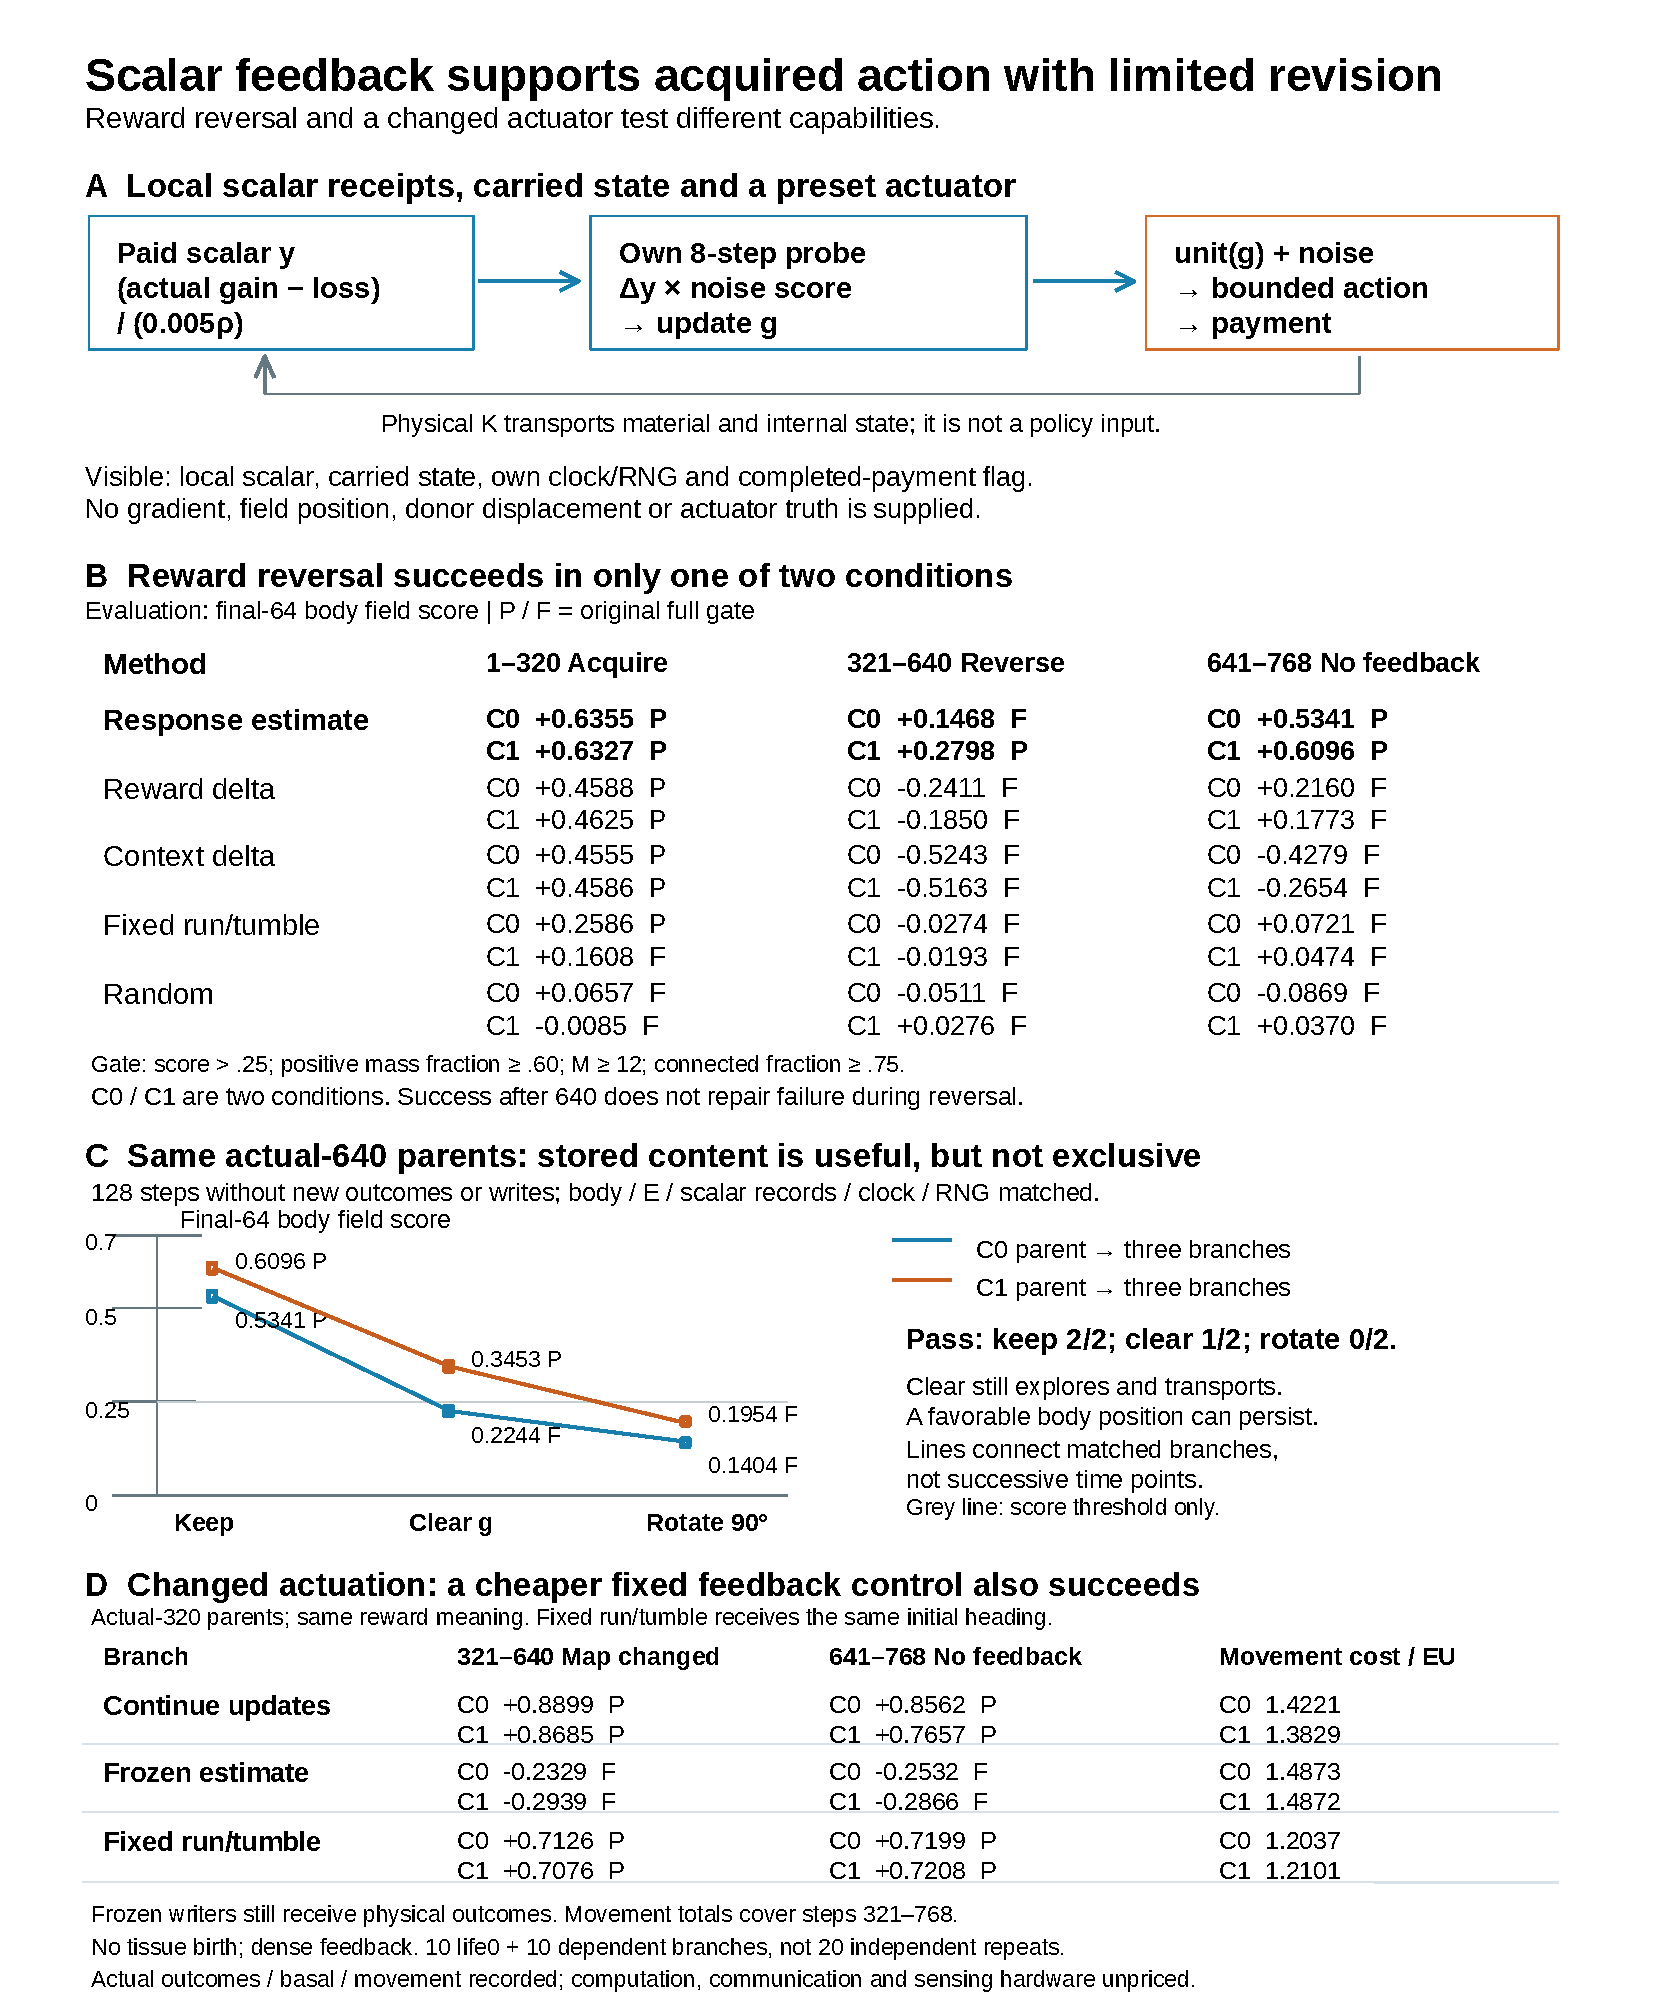
\includegraphics[width=\linewidth,height=0.68\textheight,keepaspectratio]{work/longform_v047/figures/scalar_action_v048/scalar_action.pdf}
\captionsetup{font=footnotesize}
\caption{\textbf{Scalar-only experience supports action acquisition, with different limits under reward and execution changes.}
\textbf{a}, A standard local response estimate uses completed scalar outcome changes and physically carried perturbation records. The transport operator $K$ moves material and internal state but provides no learner-facing displacement, gradient, field coordinate or actuator truth. Motion axes, cohesion, exploration and energy measurement are supplied.
\textbf{b}, All five methods, two paired seed--actuator conditions and three phases. Cells give final-64 mass-weighted field scores and the original complete gate (P/F); these evaluation quantities are not policy inputs. Response estimation passes acquisition in both conditions, reward reversal in one and the following no-new-feedback interval in both. The later success does not revise the failed reversal.
\textbf{c}, Two actual step-640 parents with response retained, cleared or rotated. Lines join related content interventions, not successive times. Retention passes twice, clearing once and rotation never. Clear branches still explore and move; rotation preserves response norm but not each bounded command or expense. Retained tails reuse recorded trajectories without replay.
\textbf{d}, From actual step-320 parents, only the physical execution map changes. Continued estimation and fixed run/tumble both pass the paid and later no-new-feedback windows in both conditions; frozen estimation fails. The fixed control receives the same acquired initial heading and spends less on movement. Expenditure sums both continuation phases. Ten new life-zero paths and ten dependent branches are not twenty independent repetitions. The conservative host has no tissue birth; physical expense is reported without a separate tariff for computation or sensing hardware. All phase outcomes and accounts are retained in the accompanying scalar-action source tables.}
\label{fig:scalar-action}
\end{figure}



\subsection*{A continuing cellular body acquires and reverses a cue preference}

Controlled cue encounters isolate learning of an outcome relationship from learning how to direct an action. The assay keeps one deformable cellular body through acquisition, a neutral interval, an unannounced contingency reversal and a second neutral interval. Two cue channels are initially assigned opposite local feedback signs. After exposure, a probe presents the cues on opposite sides of the body without reinforcement. Later exposure reverses which cue predicts the positive outcome. The learner is not supplied with a phase label, the reversal time, the environmental mapping or a desired action. Its available signals are the local cues and the energy gain or loss actually delivered to tissue. An appropriate response must consequently depend on the experienced association rather than on a supplied task identifier.

The body is a continuous density and intracellular-energy field on a periodic $32\times32$ lattice. Local paid transport changes its spatial distribution; cohesion and pressure support a connected deformable organization. It is not a rigid particle following a prescribed centre trajectory. However, this implementation has no regenerative birth and does not use a trained Lenia growth rule. The sensing channels, cohesion, cue-gradient actuator and conversion of local energy feedback into a signed teaching signal are supplied components. The experiment tests whether plastic state can acquire and revise the relation between those channels and outcomes within a continuing body; it does not test the emergence of the sensors, actuator or learning rule.

Three update conditions share these bodily dynamics. A non-plastic reactor retains its initial cue values. A strong recent-feedback rule updates the value of the most recently registered cue with unit learning rate. An eligibility-trace rule updates values using a decaying local cue trace and learning rate $0.5$. Both plastic rules use a normalized prediction error based on realized local feedback. Values and their associated cue records travel with the actual tissue transport. Their use follows established ideas of associative updates and eligibility\cite{sutton,florian,izhikevich,fremaux}; implementing these ideas locally in the present body is not, by itself, an algorithmic invention.

The completed assay contains two random seeds and both orders of the initial cue--feedback mapping. These give four related seed--order conditions per arm and pairing condition. There are 24 continuing 960-step life trajectories, followed by 24 value-preserving and 24 value-erased continuations. The latter are paired forks of the same terminal bodies, not additional independent acquisition histories. All 72 paths remain alive under the specified mass and connectivity criterion. The four seed--order conditions should not be described as four independent random seeds, and the many local cue contacts are not independent biological replicates.

With paired feedback, both plastic rules show strong appropriate cue contact after acquisition (Fig.~\ref{fig:lifetime-learning}). The endpoint contact fraction at the first acquisition probe averages $0.999993$ for the recent-feedback rule and $0.999993$ for the eligibility rule, compared with approximately $0.5$ for the reactor. Following a neutral interval, the corresponding means remain $0.999967$ and $0.999996$. These fractions measure the share of actual probe contact assigned to the currently correct cue, rather than a classification score computed directly from the internal values. They therefore include the body's movement and spatial encounter with the two probe regions.

After the cue--feedback relation reverses, both plastic rules redirect contact towards the newly positive cue. Their first post-reversal probe means are $0.999994$ and $0.999986$. At the final retention probe, the recent-feedback mean is $0.989435$, with individual values from $0.978865$ to $0.999998$, and the eligibility mean is $0.999998$, with values from $0.999997$ to $0.999999$. The result establishes re-acquisition after an unannounced change within this protocol. It does not establish immediate reversal upon the environmental change, nor transfer to arbitrary cue schedules, geometries or resource regimes. The first post-reversal probe follows eight completed feedback pulses, four for each cue. No independent choice score was recorded during forced exposure, so recovery after a single feedback event is not established.

Pairing controls are essential to this interpretation. Unpaired exposures retain the cue and feedback opportunities but balance positive and negative feedback for each cue. Across opposite mapping orders their mean correct-contact fraction is approximately $0.5$. This aggregate does not mean that every unpaired body remains indifferent. Some unpaired acquisition probes show nearly exclusive contact with one cue, producing very small or very large correct-contact fractions depending on the assigned mapping. At the final reversal-retention probe, unpaired eligibility values span approximately $0.0164$ to $0.9836$. The pairing comparison therefore identifies the usefulness of experienced cue--outcome correspondence across the tested conditions; it does not equate absence of reliable correspondence with absence of an internally acquired preference.

\begin{figure}[p]
\centering
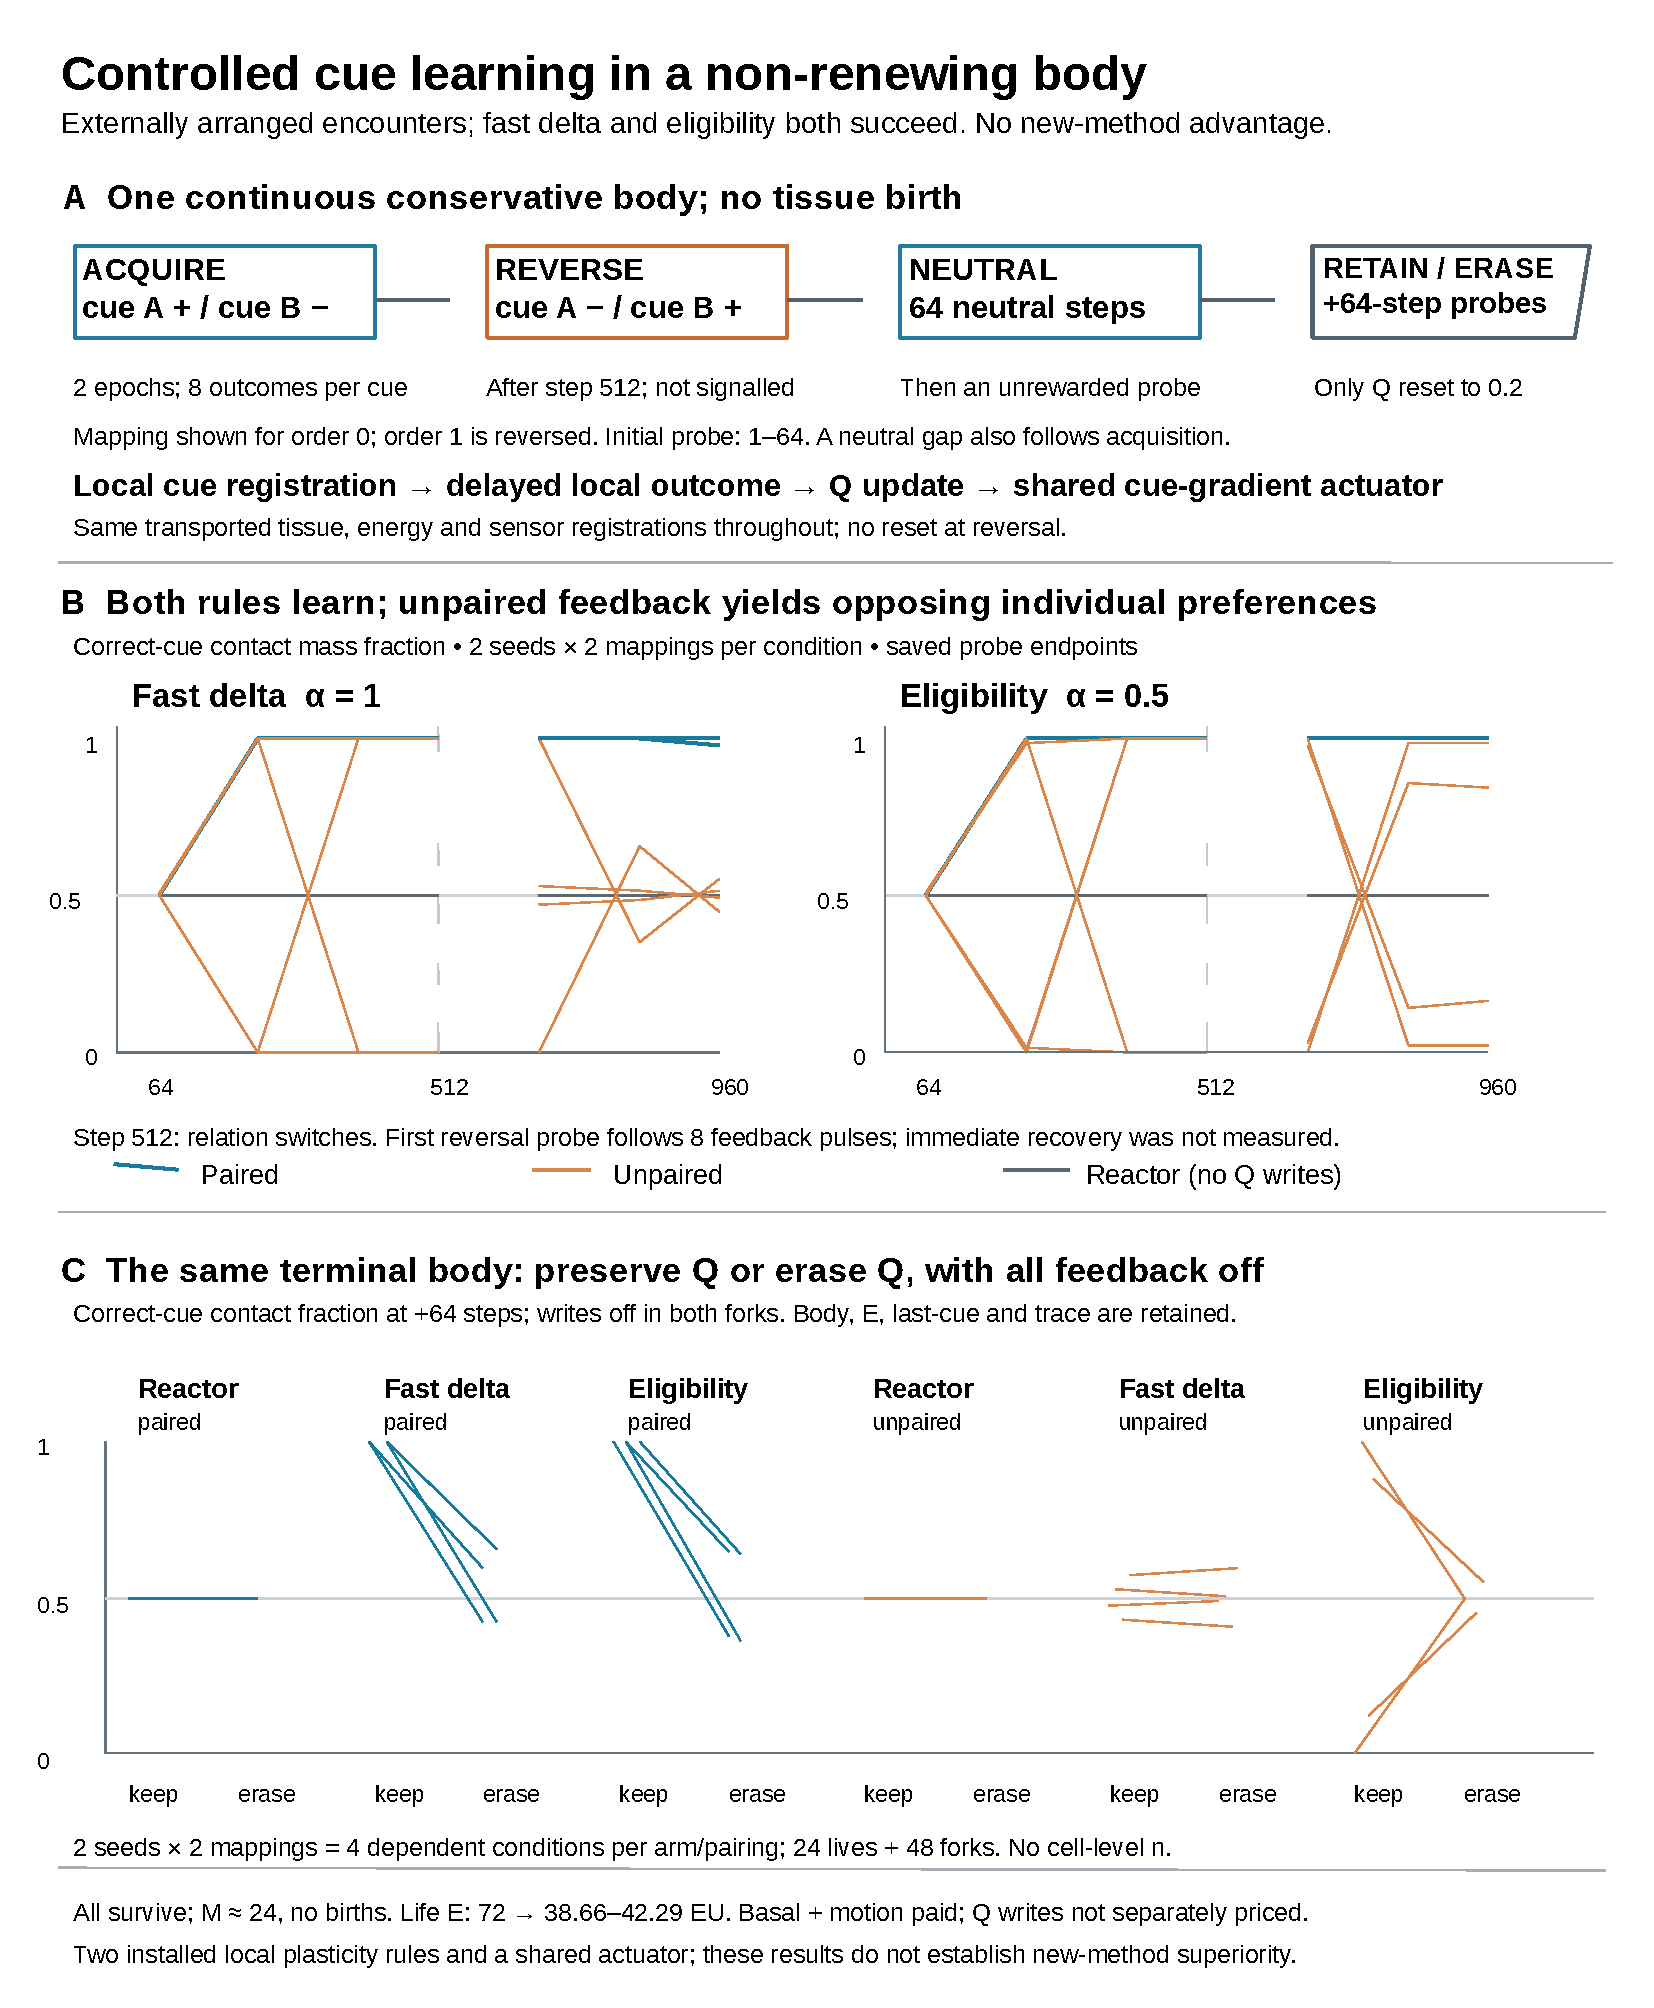
\includegraphics[width=\linewidth,height=.76\textheight,keepaspectratio]{work/longform_v047/figures/lifetime_learning_v0474/lifetime_learning.pdf}
\caption{\textbf{Controlled cue learning in a non-renewing body.}
\textbf{a}, Externally arranged encounters on one continuing conservative body, without tissue birth. \textbf{b}, Two installed update rules, recent-feedback (fast delta) and eligibility, acquire and reverse cue preference in a continuing transported body. Four related seed--mapping paths per condition retain the individual outcomes: the unpaired mean near one half hides opposing preferences. \textbf{c}, Matched terminal freeze/erase forks change only the initial stored cue values, preserving body, energy and sensory registrations at branching. The first reversal probe follows eight new feedback pulses. All paths survive in this no-birth host, while movement and basal costs reduce available energy. Neither update rule establishes a new-method advantage. Values are actual probe contact fractions; repeated phases and terminal forks are not independent histories.}
\label{fig:lifetime-learning}
\end{figure}


\subsection*{Erasure reduces preference, while successful behaviour still has a physical cost}

To test expression after acquisition, each terminal body is continued for another 64 unreinforced steps with value writing disabled. One branch retains its learned cue values, and the other resets those values to the common initial value of $0.2$. Density, energy, cue traces and the rest of the terminal bodily state are retained. This is a targeted value-erasure comparison at a shared state, rather than a replay of acquisition or a replacement of the whole body with a naive initialization.

In paired recent-feedback bodies, the value-preserving branch reaches a mean appropriate-contact fraction of $0.9999997$, whereas erasure reduces it to $0.5211$; individual erased outcomes range from $0.4194$ to $0.6533$. In paired eligibility bodies, the corresponding means are $0.9999988$ and $0.5075$, with erased outcomes from $0.3618$ to $0.6494$. The comparison supports a role for the stored values in expression during this terminal probe. Values are not the only history-dependent part of the body: erasure leaves the acquired geometry, energy distribution and other local records in place. The residual spread after erasure is thus informative, and should not be rounded into a claim of exact restoration of a pristine naive state.

The behavioural gain occurs in a body that continues to pay for movement and basal activity. Mean movement expenditure across paired 960-step lives is $3.4661$ for recent feedback and $3.3788$ for eligibility, compared with $2.1551$ for the reactor. Basal expenditure is $27.648$ in all these groups. Actual feedback gains and losses also differ because the bodies evolve differently during exposure. Mean terminal energy is $42.0836$ for paired recent feedback, $41.9749$ for paired eligibility and $42.1969$ for the paired reactor. Thus successful cue choice does not require a larger final energy reserve than the non-plastic control. A screening rule demanding simultaneous improvement in behaviour and every bodily total would reject this meaningful behavioural change for the wrong reason.

This does not remove the need for physical accounting. The result is bounded by the viability of the actual body and by the resources supplied in the protocol. Initial mass and energy are 24 and 72; no starvation or injury loss occurs in these runs, and movement payments are met. The reported energy account closes to numerical precision. However, the additional arithmetic required to update and read values is not separately assigned a physical energy cost. The assay therefore measures movement and basal costs under its specified model, rather than the complete thermodynamic cost of learning. It also provides no evidence that the body can replenish its material indefinitely: the continuing body is conservative and has no birth process.

The recent-feedback control is deliberately strong. It can retain the latest cue through the delayed feedback interval and use that record to update values rapidly. Its success means that the present delay structure does not establish an advantage of the eligibility rule. The small difference at the final retention probe is not a basis for declaring a general superiority, given two seeds, related mapping orders and highly saturated probe performance. The experiment instead supplies a usable behavioural benchmark: acquired preference, reversal and retention are observable within one continuing cellular body, while matched non-plastic, unpaired and erasure controls limit alternative explanations. Longer or conflicting delays, unfamiliar contexts and concurrent bodily replacement remain distinct questions.

\subsection*{Changing which past event predicts feedback requires temporal credit reassignment}

The success of recent feedback in the controlled cue assay leaves an important ambiguity: remembering the latest cue may suffice because no competing cue intervenes before its outcome. A second experiment separates the information in recent and earlier contact. Each lesson presents one cue, a brief gap, a statistically independent second cue and another gap before local feedback. All four earlier--recent cue combinations occur within each block. Initially the earlier cue determines the outcome. The body must therefore retain information across a distractor rather than merely respond to the last event (Fig.~\ref{fig:temporal-credit}).

Five update conditions share the physical host and visible local records. Recent-cue delta uses the latest registered event; a fixed exponential trace mixes recent experience; a fixed earlier-event delta uses the known task lag; joint delta learns four coefficients over both cue identities at both lags; and a two-expert gate adjusts the weight assigned to the two temporal sources from their local prediction errors. The fixed earlier-event control is deliberately informed about the original delay structure. Joint delta and the gate receive both records but no instruction identifying which one determines feedback. The gate is an established type of error-weighted combination, not a claim of a newly discovered learning algorithm.

Two new seeds and two initial cue-meaning orders give four conditions per rule. Fixed earlier-event delta, joint delta and the gated experts each pass all six acquisition, meaning-reversal and retention probes in all four conditions, with the continuing bodies alive. Recent-cue delta and the particular fixed trace tested here each pass the complete six-probe sequence in zero of four conditions. One recent-cue life and two fixed-trace lives fail the predefined connectivity condition; their mass remains near 24 and energy remains positive. These are losses of the required connected individual, not total material extinction. Incomplete and unobserved probes remain incomplete or missing. The negative result for this exponential trace does not establish failure of eligibility traces in general.

The harder continuation changes the predictive temporal source without changing the cue identities' positive and negative meanings. At step 1216, all seventeen surviving complete physical states continue without resetting their bodies, value banks, traces or cue registrations. The most recent event now determines feedback. Each rule inherits its own actual acquired history, so cross-rule comparisons include the different bodies and internal states produced earlier. They are not algorithm substitutions into one identical parent. The three previously failed lives remain failed and are not restarted.

Joint delta and the gate pass all three prescribed probes in all four continued conditions. The fixed earlier-event rule fails at least one probe in every condition. Its two seed-7403 paths retain the wrong preference at the final retention probe; both seed-7404 paths recover after an initial probe near $0.48$. The surviving recent-cue and fixed-trace subsets pass three of three and two of two continuations, respectively. These subset successes are expected to become possible when recent contact is now relevant, but they do not erase the earlier failures or become four-of-four success over the complete history.

\begin{figure}[p]
\centering
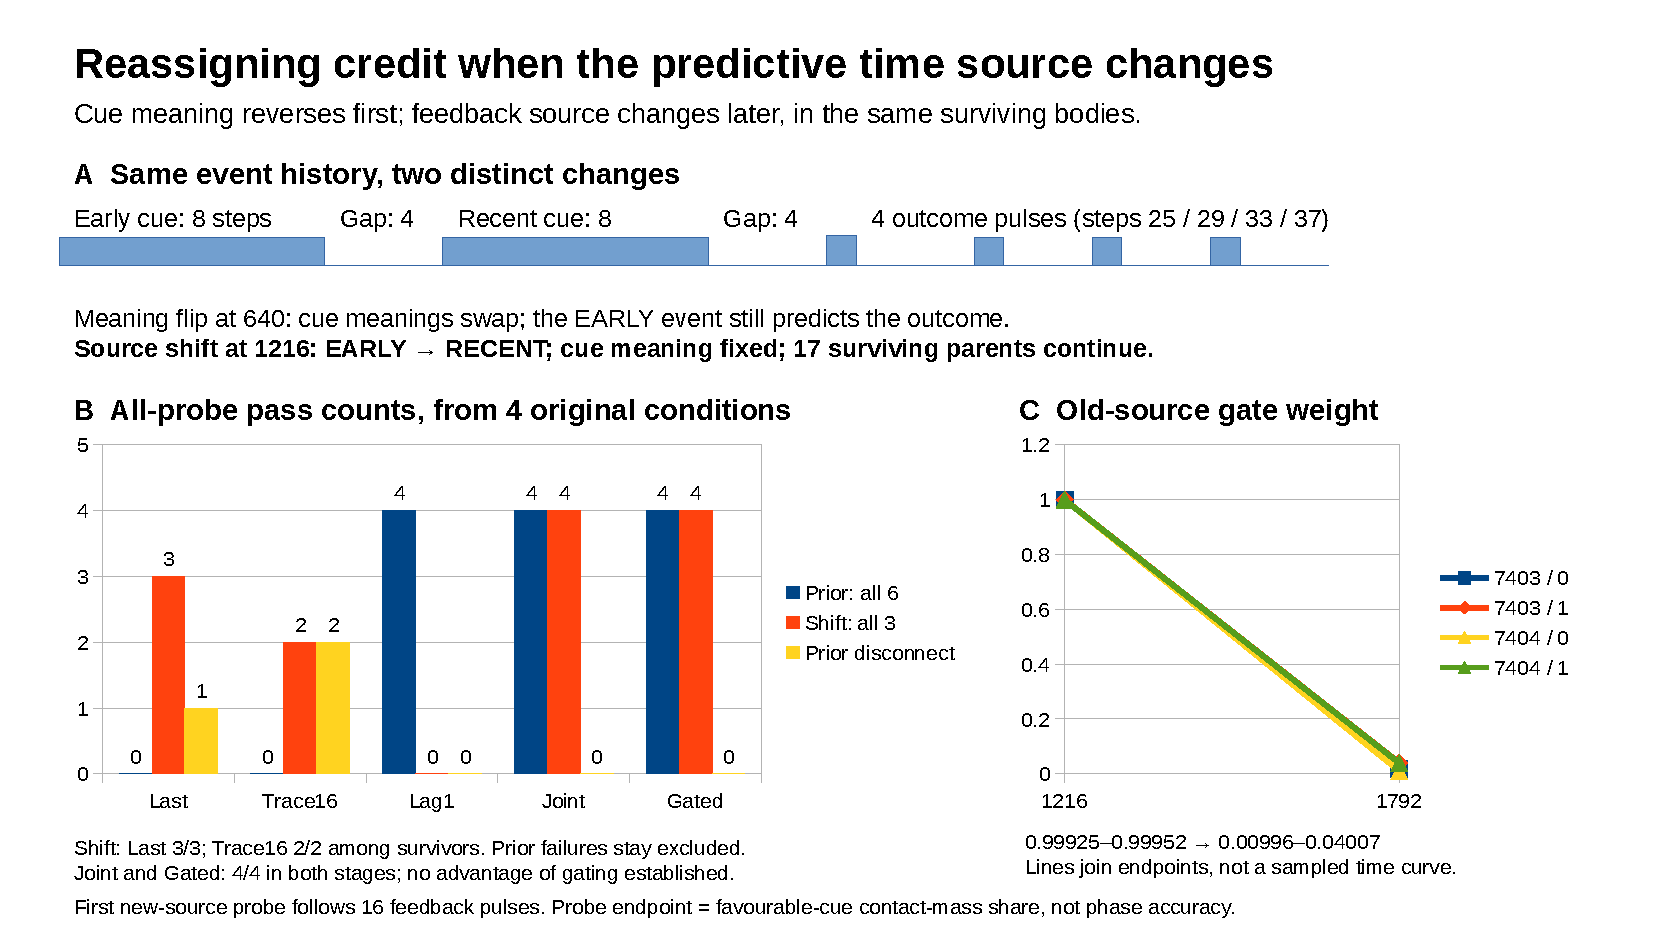
\includegraphics[width=\linewidth,height=.76\textheight,keepaspectratio]{work/longform_v047/figures/temporal_credit/temporal_credit.pdf}
\caption{\textbf{Useful history changes when the predictive temporal source changes.}
\textbf{A}, An independent intervening cue separates earlier from recent contact. The first change reverses cue meaning; the later change makes the recent event predictive while preserving cue meaning. Seventeen surviving bodies continue without reset. \textbf{B}, Fixed earlier-event delta, joint delta and gated experts pass all six initial acquisition, reversal and retention probes in four related seed--order conditions. Joint delta and gated experts also pass all three later probes in four of four conditions; fixed earlier-event delta fails a phase in all four. Earlier connectivity failures in recent-cue delta and the fixed trace remain failures. Their later three-of-three and two-of-two successes describe surviving subsets, shown relative to the original four-condition count. \textbf{C}, Individual gated-rule weights shift from the earlier to the recent source. Lines join the two measured endpoints and do not depict the intervening time course. Joint delta achieves the same behavioural coverage. Probe values are favourable-cue contact-mass fractions at the final frame; the first changed-source probe follows sixteen feedback pulses. These conservative bodies do not regenerate tissue, and additional learning arithmetic is not physically priced.}
\label{fig:temporal-credit}
\end{figure}


The gate supplies a direct internal readout of temporal reassignment. Across its four paths, the body-weighted earlier-source weight changes from $0.99925$--$0.99952$ at the boundary to $0.00996$--$0.04007$ after the changed-source continuation. This is a change between two available temporal hypotheses, driven by experienced local outcomes. Joint delta achieves the same behavioural coverage without an explicit gate, however, so successful reassignment does not establish that the gated architecture is necessary or superior. Terminal energy and movement costs also differ across paths: joint-delta energy ranges from $14.34$ to $17.83$, and gated energy from $13.91$ to $17.18$, with overlapping movement-expenditure ranges. The analysis retains these physical consequences without demanding that every cost or reserve improve for learned behaviour to count.

The measurements resolve a finite capability, not instantaneous adaptation. The first new-source feedback arrives after 24 updates without an informative new outcome. The first subsequent choice probe occurs after sixteen feedback pulses. Probe scores are the favourable-cue share of contact mass at the probe's last frame, not the proportion of correct decisions across the entire exposure stage. Following the changed relation, neutral intervals and matched value-freeze and association-erasure forks again distinguish retained expression from continued correction. Erasure reduces the learned preferences but leaves body, energy and sensory history intact; residual preferences cannot be called erasure of all memory.

These comparisons advance the behavioural question from fixed cue association to selection between past sources of evidence. They also show what has not advanced: sufficient simple joint history already solves the tested problem. The lessons and actuator remain supplied, broad training fields permit feedback at weak contact, the material host has no birth, and controller arithmetic and storage are not physically charged. Self-generated experience in a fixed arena and retention through regeneration remain open. The continuous actual animation preserves the old and changed-source segments, including the stopped histories, so the claim rests on continuing bodies rather than resetting an agent for each successful phase.

\subsection*{Historical content can determine action while a simple history table matches the capability}

A separate conservative body tests a different informational requirement: choosing between actions when the current cue is the same but earlier cue order differs. Opposite early orders are paired with identical terminal cue, GO signal, gap positions and total duration. Only the value of the actually executed action is updated from completed reward or punishment; unselected action values are unchanged. The complete literal-history control has a 16-event buffer and a 128-entry table, sufficient for all twelve legal strings. A second six-entry table uses a fixed filter that removes gap events. A fixed encoding of the current full bodily field with a linear action-value readout supplies a third, restricted comparator. History storage, the START boundary, cue delivery and action readout are central external components of this assay, distinct from the distributed scalar-action learner.

Across three actual seed histories, the literal and filtered tables each make all 36 test choices correctly before the relationship changes and all 36 correctly after retraining. During the changed acquisition stage, the literal table makes 36 of 72 choices correctly and the filtered table 54 of 72. Filtering also leaves higher terminal energy. The benefit is consistent with a supplied invariance reducing the number of distinct strings to relearn, rather than a new predictive-state mechanism. The tested current-body readout achieves 19/36 and 17/36 in the two frozen tests. This result limits that encoding and readout; it does not show that every legitimate use of bodily state must fail (Table~\ref{tab:history-main}). These tests retain learned strings; they do not establish new gap-length generalization.

Actual content interventions make the distinction between history use and representation innovation concrete. From complete saved parents, we exchange only the two early central cue records while preserving the learned table and the current body. Each table changes from 6/6 correct choices to 0/6, and all twelve actual motor commands change; none of the six commands under the current-body readout changes. Historical content therefore affects action, yet the simple complete-history control already expresses the relevant capability. The nine continuous strategy paths share three seed histories, and the eighteen intervention futures are dependent branches. The series contains 7,236 actual bodily steps. The 108 intervention steps completed before a final file-size assertion failed against the worker's self-imposed 8 MiB limit; preserved complete states and receipts support their analysis, while the failed packaging status remains explicit (Supplementary Tables~\ref{tab:history-stages} and \ref{tab:history-content}).

\begingroup\small
\begin{longtable}{lllll}
\caption{Selected-action learning under three supplied history encodings. Entries are correct choices/actual episodes across the three paired seed histories. A: acquisition; H: frozen-write test; C: changed relation with learning; HC: frozen-write test of that relation. Test outcomes are still physically paid. Episode counts are not independent experimental replicates.}\label{tab:history-main}\\
\toprule
Representation & A & H & C & HC \\
\midrule
\endfirsthead
\toprule
Representation & A & H & C & HC \\
\midrule
\endhead
Literal & 54/72 & 36/36 & 36/72 & 36/36 \\
Filtered & 63/72 & 36/36 & 54/72 & 36/36 \\
Body readout & 35/72 & 19/36 & 34/72 & 17/36 \\
\bottomrule
\end{longtable}
\endgroup


\subsection*{Material-carried history supports learned choices without an advantage from plastic recurrent gain}

The central-history comparison leaves a different question: can useful history remain in local states carried by actual tissue, and must the dynamics of that memory themselves be learned? A separate conservative body carries its history, local readout weights and eligibility records through the same material transport and mixing as its density. Locally paid cue contact and completed energy consequences update those quantities. There is no START clearing. A fixed common whole-body readout and motor interface turn the local values into a paid choice; these components are supplied, so success does not demonstrate acquisition of the actuator tested in the scalar-action experiment.

We compare a standard adaptive recurrent gain with fixed local dynamics and a strong central history table. The first complete comparison exposes a closed-loop access failure: biased local actions carry the body away from the stationary stimulus region, so later cues and outcomes are often not received. Those failures remain failures, but missing feedback cannot establish that an adequately supplied local state is intrinsically unlearnable. A second comparison adds six actual, paid return-to-station updates after every assay for all policies. It restores all 384 scheduled feedback episodes. Both seed histories in that comparison happen to begin with the positive mapping, however, and the fixed local delay line already answers most initial patterns by its initial majority readout. Its 48/48 acquisition score is therefore insufficient evidence that the outcome relationship was learned.

A separately frozen comparison counterbalances the initial mapping across two new seed histories without retuning the learning rule. The six-event local delay line with ordinary online delta readout obtains 60/64 acquisition choices, including 28/32 under the initially negative mapping. It then makes all 16 choices correctly with previously unseen blank intervals and all 16 after reversal and retraining. The central history table also achieves 16/16 in both tests. The adaptive-gain candidate achieves 10/16 and 8/16, respectively. Errors during the changed-relation learning period remain in the denominator: local delay, central table and adaptive gain obtain 13/32, 16/32 and 9/32. Neither perfect later retention nor an unknown reversal can erase these recorded errors (Table~\ref{tab:local-history-main}).

At prespecified complete parents, we also alter history content while preserving the current body, energy and readout. Negating local delay content changes three of four actual paid actions and changes correctness from 3/4 to 0/4; the corresponding central-table intervention changes four of four. Restoring the adaptive gain to its initial value is nonzero in all four selected parents but changes none of their actions, leaving correctness at 2/4. A sham continuation reproduces the complete state exactly. These limited interventions establish a contribution of some stored histories, while supplying no evidence that the acquired recurrent gain is necessary. They are dependent branches of existing histories, not additional learned lives.

The distinction between content and dynamics now has a physical instance: fixed material-carried memory plus a learned local readout is sufficient under the paid return protocol. The adaptive-gain implementation has fourteen local fields, whereas the fixed delay implementation has twenty-two; the central control has a six-event record and a 128-entry table. Equal information capacity or full physical computation cost is not claimed. All movement, return, local sensing, upkeep and assay charges remain in Supplementary Tables~\ref{tab:local-history-stages}--\ref{tab:local-history-jobs}. The complete series contains six comparative seed histories plus one opportunity history, twenty-three continuous strategy paths and twenty-one dependent probes, totalling 23,491 actual cellular updates. This negative result closes the extra-value claim for the tested gain candidate, not the possibility that other bodily memory dynamics could be learned.

\begingroup\small
\begin{longtable}{lllll}
\caption{Balanced initial mappings in the material-carried-history assay. Entries pool correct/actual episodes across two paired seed histories, not independent episode replicates. A: acquisition; G: unfamiliar blank intervals; R: changed-relation learning; HG: retained choices after retraining with unfamiliar intervals. All feedback is physically delivered. Gain, Delay and Table denote adaptive recurrent gain, fixed six-event local memory and the central history table.}\label{tab:local-history-main}\\
\toprule
Memory/readout & A & G & R & HG \\
\midrule
\endfirsthead
\toprule
Memory/readout & A & G & R & HG \\
\midrule
\endhead
Gain & 30/64 & 10/16 & 9/32 & 8/16 \\
Delay & 60/64 & 16/16 & 13/32 & 16/16 \\
Table & 56/64 & 16/16 & 16/32 & 16/16 \\
\bottomrule
\end{longtable}
\endgroup


\subsection*{A learned material coefficient can be exactly matched by a fixed-material readout}

A further conservative-body comparison asks whether putting acquired content directly into a physical response coefficient adds a capability beyond ordinary online readout. Each site's bounded compliance coefficient $c$ changes both passive local forces and transport under an externally applied load through $M(c)=(1+|c|)^{-1}\left(\begin{smallmatrix}1&c\\c&1\end{smallmatrix}\right)$. The coefficient is physically carried and mixed. Standard delta and last-outcome rules update it from completed local movement and actual energy consequences. This assay supplies a movement observation and a paid centring fixture, so it is a more informative, externally supported interface than the primary scalar-only learner.

Across three main histories, the delta rule's held-out scores are approximately $0.811$, $0.797$ and $0.788$ after acquisition and the two relationship changes. These scores retain all registered mass-time in the denominator. Conditional accuracy is near $0.998$, but only about $0.79$--$0.81$ of registered mass-time is eligible; reporting only the conditional value would hide that incomplete coverage. Last-outcome learning has similar performance, while immediate feedback and passive hysteresis perform less well under the declared tests (Supplementary Table~\ref{tab:physical-state-stages}).

The fixed-material control supplies the decisive explanation. Unit material with a local learned readout $w$ applies the additional force $(M(w)-I)f$. Under the same local force information, range and parameter tariff, $If+(M(w)-I)f=M(w)f$. Thus the common interface allows an algebraically equivalent implementation. Its three actual body, energy, behaviour and expense histories match delta compliance to a maximum recorded scalar discrepancy of $4.27\times10^{-14}$. There is no extra demonstrated capability or efficiency from assigning the same learned coefficient to the material law.

Six prespecified complete acquired/revised parents support paired physical interventions. Reversing only $c$ preserves density and energy pointwise, as well as the magnitudes of the tensor eigenvalues, while reducing registered correct-contact scores from $0.739$--$0.849$ to $0.00053$--$0.00276$. Content therefore affects the present response. After $c$ is cleared, conditional correctness is only $0.465$--$0.537$; the original density shape outperforms its mass/energy-matched mirror in only two of six cases. These probes do not support stable useful memory in the residual density geometry. Clearing also changes the constitutive mechanics, so its failure alone would not be a memory-specific lesion. A full-state sham is exact. The strong equivalent readout, acquired/revised trajectories and sign intervention together establish a useful standard response while closing the proposed extra-value claim for this linear-compliance implementation.

\subsection*{Local feedback leaves useful contact-network content without an advantage over force compensation}

An independently supported elastic network tests whether the equivalence above is peculiar to a lattice transport coefficient. This auxiliary host contains fifteen existing material units connected only by actual near contact. Changing a connection's rest length changes the forces on its two endpoints. It is not a cellular automaton, has no tissue birth, and receives a fixed left support and a periodic rightward load. Its task is resource uptake under a spatially shifted supply, not acquisition of autonomous locomotion. A standard local perturbation rule adjusts rest lengths from the uptake already received at the connection's endpoints, without a supplied target direction or resource-band location.

Across three main histories, plastic rest lengths yield mean uptake 2.27404 during the first 48-step stopped-writing window and 0.75034 after the resource shift, compared with 2.09823 and 0.29758 for fixed parameters. A stronger control, however, uses fixed reference springs plus local compensating forces and matches the plastic body's complete recorded state within $8.9\times10^{-16}$. Plastic bodies also end with mean energy 50.42232, compared with 65.40015 for the fixed-parameter control. Increased uptake therefore supplies neither a net resource advantage nor additional capability beyond the force-equivalent readout. The main plastic candidate creates no new contacts after its initial network forms and breaks none; sign updates and passive creep can disconnect material despite total mass remaining fifteen (Supplementary Tables~\ref{tab:contact-stages}--\ref{tab:contact-ledger-extra}).

Three further histories compare long-term updating with the same random material perturbations but no long-term update. All three first hold windows favour updating, by 0.04866, 0.19341 and 0.06673 uptake units. After the supply shift, the differences are 0.11448, $-0.10138$ and 0.02805: only two remain positive. Six complete acquired/revised parents then supply thirteen dependent probes. Removing only the long-term rest-length offset reduces uptake in five parents and improves it in one. Preserving the old effective forces in a local compensating readout restores uptake in all six. The intervention preserves position and current perturbation initially but pays the positive change in elastic energy and a parameter-change charge, so it also changes endpoint energy; it is not a mechanically neutral memory lesion. The exact sham, independent content-use comparisons and force compensation together support a small useful contribution from ordinary locally acquired content, without establishing robust revision, learned topology or an extra material method (Supplementary Tables~\ref{tab:contact-pairs}--\ref{tab:contact-null}).


\subsection*{Contact feedback can arrive without being used effectively}

A further six-batch experiment separates access to consequences from the ability to exploit them in the same class of moving-node elastic host. Resource uptake at distal material emits a signal that travels at most one actual contact per update. In the opportunity run, the first uptake occurs at postclock 53 and the first proximal signal at 56, although the proximal material never takes up resource itself. Cutting only information transmission across a section in three actual parents preserves every recorded physical variable during 96 stopped-writing updates. The residual local signal is not erased. With writing enabled, the cut-minus-open uptake changes are tiny and of mixed sign; nearly full distal stores prevent this comparison from establishing a useful communication benefit (Supplementary Tables~\ref{tab:reach-means} and \ref{tab:reach-cut}).

Useful action consequences nevertheless exist. Three new bodies receive an actual 96-step resource-free prefix, then paid positive or negative proximal rest-length changes. Positive-minus-negative uptake is positive in all three bodies at resource position 5.4 (0.44420--0.45451) and negative at position 4.7 ($-0.42971$ to $-0.41614$). The received local signals retain the corresponding ordering. These are executed fixed-action comparisons, not counterfactual labels supplied to the learner, and they establish neither online credit assignment nor a unique causal role for one contact (Supplementary Table~\ref{tab:reach-actions}).

Providing reachable consequences does not make the tested ordinary rule reliably useful. Mean-age alignment lowers changed-environment uptake in all three histories compared with ordinary diffusion (means 0.75176 versus 1.23979). Holding actions for 96 instead of 24 updates improves that uptake in only one of three further histories; its higher terminal energy accompanies fewer paid parameter changes. Finally, three independent sparse-resource histories keep distal stores below capacity, yet diffusion yields less changed-environment uptake than no signal in all three, by 0.00542, 0.01881 and 0.00635 units. Instantaneous global feedback is not consistently better either. These unequal-information controls expose a failure of utilization under the tested rule, rather than a general absence of accessible consequences or a fair ranking of learning algorithms. Fixed material with a compensating readout exactly reproduces the first-batch physical states. Neither a new transmission-method advantage nor a broad impossibility of contact-mediated learning follows (Supplementary Tables~\ref{tab:reach-pairs}--\ref{tab:reach-jobs}).



\subsection*{Access to new evidence and expression of an acquired value are separable}

The staged lessons establish that local experience can change behaviour, but they supply encounters independently of the body's success in finding them. We therefore examine a completed fixed-field continuation of the research programme. Two cue patches are fixed before life begins, and only material inside their finite contact regions can receive positive or negative energy feedback. A shared, explicitly supplied exploratory polarity acts in all rules. The fields never follow the body's centre, and no lesson forces a particular encounter. This changes the source of experience: the body's own motion now determines which outcomes can update its local associations.

Across two mirrored seed--layout settings and two initial cue meanings, fast delta and joint delta each acquire the initially favourable contact in four of four conditions and remain viable through 1536 updates (Table~\ref{tab:self-contact}). Both pass the first unreinforced retention window. The non-writing reactor eventually fails in all four conditions, including two in which early favourable contact occurred without learning. Initial movement and sensory transduction remain supplied capabilities; the result concerns their experience-dependent redirection.

Unannounced reversal is less reliable. Each plastic rule passes the final reversal window in only two of four conditions. Joint delta then retains favourable contact in those two conditions, whereas fast delta fails the later retention window in all four. The two surviving fast-delta failures after successful reversal have substantial contact but a favourable share near $0.00225$: they express the wrong preference. The other four plastic failures, shared by both rules, have inadequate contact with either patch. They must not be classified solely from a conditional contact ratio that can approach one when its absolute support is tiny.

The feedback records make this distinction consequential. Two joint-delta bodies receive no positive payment throughout the changed-meaning interval; the corresponding fast-delta bodies receive many tiny positive payments but never satisfy the final contact-coverage requirement. Avoidance acquired earlier can thus leave a continuing body with little useful corrective experience. This is a limitation of the coupled behaviour--experience process, rather than an isolated test of a learning update supplied with equivalent evidence. Successful reacquisition is first observed after 128 paid-feedback updates, not after one outcome.

Memory expression also depends on what the test leaves intact. At the first retention boundary, all eight learning bodies supply matched association-freeze and association-erase probes. Both branches pass in all eight pairs. Keeping the same body and location near an already reached patch allows short-window performance after erasure; these probes do not isolate association-dependent retention. The conditional later advantage of joint delta likewise does not establish a general algorithmic advantage or a capacity-matched comparison. Joint-delta bodies in its two successful final conditions pay about $7.69$ energy units for movement, compared with $4.72$ for fast delta, while ending with more stored energy. The extra movement is a measured cost of this behaviour, not a reason to discard its benefit. Learning arithmetic remains unpriced, and these bodies still produce no new tissue.

\begin{table}[p]
\centering\small
\caption{\textbf{Fixed-field acquisition and reversal retain condition-specific failures.} Each row is one actual continuing body. Seed 7503 uses layout 0 and seed 7504 uses its mirror, layout 1; the full seeds are 202610197503 and 202610197504. Meaning is the initially favourable cue index. A and H1 denote initial acquisition and its retention; R and H2 denote reversal and its retention. A pass requires both favourable contact share and sufficient absolute contact, under the predeclared window rules in Methods. Dashes denote stages not obtained after stopping, rather than reconstructed outcomes. Final survival is evaluated separately.}
\label{tab:self-contact}
\begin{tabular}{lllrccccc}
\toprule
Seed & Meaning & Rule & Last step & A & H1 & R & H2 & Alive\\
\midrule
7503 & 0 & Reactor & 327 & Fail & -- & -- & -- & No\\
7503 & 0 & Fast delta & 1536 & Pass & Pass & Fail & Fail & Yes\\
7503 & 0 & Joint delta & 1536 & Pass & Pass & Fail & Fail & Yes\\
7503 & 1 & Reactor & 1146 & Pass & Pass & Fail & -- & No\\
7503 & 1 & Fast delta & 1536 & Pass & Pass & Pass & Fail & Yes\\
7503 & 1 & Joint delta & 1536 & Pass & Pass & Pass & Pass & Yes\\
7504 & 0 & Reactor & 327 & Fail & -- & -- & -- & No\\
7504 & 0 & Fast delta & 1536 & Pass & Pass & Fail & Fail & Yes\\
7504 & 0 & Joint delta & 1536 & Pass & Pass & Fail & Fail & Yes\\
7504 & 1 & Reactor & 1146 & Pass & Pass & Fail & -- & No\\
7504 & 1 & Fast delta & 1536 & Pass & Pass & Pass & Fail & Yes\\
7504 & 1 & Joint delta & 1536 & Pass & Pass & Pass & Pass & Yes\\
\bottomrule
\end{tabular}
\end{table}

\FloatBarrier

\paragraph{Matched readout interventions distinguish expression from return.}

Does failure to re-encounter a resource mean that no useful association can be expressed? Two continuations separate access to feedback from its later use. Starting from four actual surviving fixed-field bodies, a shared exploratory turn preserves connectivity for eight write/freeze branches over 512 updates, whereas the eight original-polarity branches stop after 46--61 updates under the connectivity rule, despite retaining mass 24. All sixteen branches receive zero positive or negative payment. Their eight matched write/freeze pairs remain exactly identical. This absence of a learning opportunity cannot diagnose an ineffective association update; turning alone does not restore contact with the payment regions.

A subsequent intervention temporarily removes the association-to-action contribution while leaving sensation, traces, learning inputs, the underlying actuator and prices intact. Four actual surviving parents each supply original-readout and paused-readout branches, paired with continued or frozen association updates. During the 384-step pause, the four paired conditions regain 124--125 updates with total contact mass at least $0.24$ and 381--382 positive payments. Contact with the favourable region alone never reaches $0.24$. At actual clock 2432, the write/freeze bodies have bitwise-identical density, energy, traces, polarity and sensory registers; their saved physical and payment histories also agree throughout the pause. Only the associative values and their associated coefficient bank differ. Thus the ensuing comparison concerns the joint associative state under a matched physical state, rather than conflating that state with an already different body.

Restoring the original readout for 128 updates without feedback reveals a limited expression effect. Over the final 64 updates, favourable-region mean mass is $0.01311$--$0.01336$ with writing, compared with $1.15\times10^{-7}$--$7.67\times10^{-7}$ after frozen writing. Fast delta shows the effect alongside joint delta. Yet all sixteen branches fail the original final-window behavioural criterion: neither final feedback nor final unreinforced windows contain an update with substantial total contact. The writing branches' favourable shares of $0.697$--$0.734$ have mean total-contact denominators of only $0.01787$--$0.01915$. These window-integrated ratios are neither whole-stage accuracy nor evidence of successful return. Final stored energy is only $2.13$--$2.76$, and movement and starvation losses remain substantial (Supplementary Tables~\ref{tab:recontact-costs}--\ref{tab:readout-expression}). The result isolates a small associative contribution to action under the supplied intervention; it does not establish autonomous recovery, a joint-delta advantage or sustainable foraging.

\subsection*{Coordinated movement and residence do not guarantee a successful complete life}

The weak-contact result leaves open whether the limitation lies in association writing or in the way local drives combine into bodily motion. A separate continuation returns to four actual clock-640 fast-delta bodies and changes only the coordination of their action signal. Current local drive, exponential temporal smoothing, the same smoothing with one occupied-neighbour propagation, and the same smoothing with a body-mass-weighted pooled signal are compared under the same local feedback rule. The pooled condition supplies centralized communication. It is a capacity reference, not a local algorithm or a mathematical upper bound. All sixteen paths remain viable through 256 further updates with the old meaning and 256 after an unannounced reversal.

Original, temporally smoothed and neighbouring signals each pass the reversal's final 64-update window in two of four conditions; pooling passes four of four. Neighbour propagation nevertheless has measurable effects. In the two initial-meaning-0 conditions its final favourable-region mean mass is $0.2021$ and $0.1967$, compared with nearly zero under temporal smoothing. Both still meet the absolute contact threshold in only 20 of 64 updates, below the required 32. In the other two conditions, the first complete recovery window ends 19 updates earlier than with temporal smoothing. Failure to improve coverage across the four conditions therefore does not imply a zero effect. Pooling yields favourable-region mean mass of $5.00$--$10.13$, about 21--42\% of the body. However, two pooled bodies had already left the formerly favourable region before reversal, so four passing endpoints alone cannot identify new learning.

We therefore branch each actual pooled clock-896 parent into continued association writing and frozen writing. The branches share the complete initial body, energy, associations, sensory records, traces, polarity and action signal. They encounter the same changed environment for 256 updates and then continue for 128 updates with both payment and writing disabled. Continued writing passes the reversal's last window in all four conditions; freezing passes two. In the two initial-meaning-0 parents, writing is required for success within this paired comparison, and its benefit persists through the final unreinforced window. In the other two parents, the frozen branch already succeeds and retains favourable contact better than continued writing. Both groups consequently pass two of four final retention windows, but these are opposite pairs of parents (Table~\ref{tab:coordinated-pairs}). Group means or equal pass counts would hide this distinction.

\begin{table}[htbp]\centering\small
\caption{Continued writing has opposite retention effects in different acquired parents. W/F are writing/frozen branches of the same pooled clock-896 state. $\overline M_g$ is mean absolute favourable-region mass in the specified final 64 updates; $f$ is the contact mass-time share. L0/L1 identify the two related seed--layout settings and $g$ the initial favourable cue. Retention is the last 64 of 128 unreinforced updates. All four W branches pass paid reversal; only initial-$g0$ W and initial-$g1$ F branches pass final retention.}\label{tab:coordinated-pairs}
\begin{tabular}{lrrr}\toprule
Parent & Reversal $\overline M_g$ W/F & Retention $\overline M_g$ W/F & Retention $f$ W/F\\\midrule
L0g0 & 10.133 / 0.348 & 4.072 / 0.039 & 0.837 / 0.070 \\
L0g1 & 5.000 / 13.007 & 0.671 / 8.722 & 0.153 / 0.915 \\
L1g0 & 9.640 / 0.317 & 3.703 / 0.041 & 0.793 / 0.074 \\
L1g1 & 4.998 / 13.002 & 0.670 / 8.716 & 0.153 / 0.914 \\
\bottomrule\end{tabular}
\end{table}
\FloatBarrier


The added behaviour has physical consequences. During paid reversal in the two conditions requiring writing, movement expenditure is approximately $0.775$ and $0.785$, versus $0.527$ and $0.517$ with freezing. Greater movement cost does not invalidate the behavioural gain. All eight continuations remain viable; final energy spans $73.72$--$85.49$ with writing and $54.09$--$86.55$ with freezing. Complete per-condition outcomes and costs are retained in Supplementary Tables~\ref{tab:coordination-outcomes}--\ref{tab:coordinated-costs}, rather than requiring every reserve and cost to improve together.

A passive account further separates retention of association content from persistence of behaviour. In all four writing branches, each cue's material-weighted association total, $\sum_x\rho_x Q_{x,c}$, changes by at most $8.9\times10^{-16}$ during the unreinforced period, while mass remains 24. Nevertheless, the two initial-meaning-1 bodies lose favourable occupancy: their final contact shares fall to approximately $0.153$. Their association totals have not been erased. This conservation does not imply unchanged local concentrations or an unchanged functional policy: position, local state, action signals and cue-driven motion still evolve. Frozen branches with material loss need not conserve the same totals. Thus these experiments support conditional relearning and short retention with a strong simple updater, while leaving sustained action and residence unresolved; they establish neither a general writing benefit nor a new local learning algorithm.

\paragraph{Residence controls and complete-life comparison.}

Does continuing propulsion carry an otherwise competent body away from a favourable region? A factorial intervention at the four actual writing states from clock 1152 retains or suppresses the complete cue drive and the exploratory polarity drive independently. All branches continue their internal state and material transport without feedback or association writing. Removing polarity while retaining cue drive increases final favourable contact in all four parents, and all four pass the finite contact criterion. However, removing both drives also passes in all four. The latter keeps cohesion and pressure active and preserves the acquired starting location; it is a low-motion physical control, not a frozen body or a learned stopping response.

The cue-only minus both-off differences in final-window favourable mean mass are $-1.481$, $+1.395$, $-1.211$ and $+1.394$ in the four ordered conditions. Cue-dependent expression therefore has opposite effects across acquired states. Removing propulsion can improve finite residence without establishing a common association advantage. All sixteen logical paths retain mass 24 and survive. Their material-weighted association totals change by at most $1.2\times10^{-15}$, while local value changes reach $0.459$--$1.145$. These measurements directly demonstrate that a conserved global total is compatible with changing local expression (Supplementary Table~\ref{tab:polarity-expression}).

To test whether stopping could instead support a complete behavioural history, an independent experiment starts new bodies at life zero. It compares the original pooled fast-delta actuator, fixed contact-dependent suppression of polarity, and suppression additionally conditional on a positive cue-weighted learned value. All three share visible cue/value information, learning, physical dynamics and prices. Acquisition lasts 512 paid updates, followed by 384 updates after an unannounced meaning reversal and 128 without feedback. These are preset actuator rules, not new learning algorithms.

Both braking rules pass acquisition, reversal and retention in two of four conditions at each stage. Crucially, those successes do not belong to the same conditions (Table~\ref{tab:brake-lives}). No life passes all three stages under either rule, and none does under the original actuator. Initial-meaning-0 bodies fail acquisition; after reversal, their formerly unfavourable location becomes favourable, permitting substantial contact and residence. Initial-meaning-1 bodies acquire the original preference but fail the final reversal and retention windows. These complementary outcomes cannot be assembled into a successful acquire--reverse--retain sequence.

\begin{table}[htbp]\centering\small
\caption{Phase-specific successes do not form a successful complete life. Entries are acquisition/reversal/retention passes (1/0) for the same life. L0/L1 denote the two new seed--layout settings and $g$ the initial favourable cue. Each phase uses its fixed final 64-update window, including absolute contact requirements. All twelve lives survive, but each method has zero of four lives passing all three phases. These contexts differ from the acquired parents in Table~\ref{tab:coordinated-pairs}.}\label{tab:brake-lives}
\begin{tabular}{lccc}\toprule
Context & Original fast delta & Fixed contact brake & Value-conditioned brake\\\midrule
L0g0 & 0/1/0 & 0/1/1 & 0/1/1 \\
L0g1 & 0/0/0 & 1/0/0 & 1/0/0 \\
L1g0 & 0/1/0 & 0/1/1 & 0/1/1 \\
L1g1 & 0/0/0 & 1/0/0 & 1/0/0 \\
\bottomrule\end{tabular}\end{table}\FloatBarrier


Transient successes also fail to establish sustained recovery. The two initial-meaning-1 value-braked bodies first complete a passing 64-update reversal window at offsets 88 and 86, but their final reversal mean favourable masses are only $0.000355$ and $0.000130$. One contact share rounds to one despite this negligible absolute amount. Conversely, value-braked initial-meaning-0 bodies retain mean favourable masses of $10.870$ and $9.917$ after feedback stops, while fixed braking retains $11.445$ and $11.622$. This is finite residence following a change in the value of an occupied location, not evidence of successful initial acquisition followed by relearning.

All twelve new lives survive, and stage-wise costs and failed windows remain part of the comparison (Supplementary Tables~\ref{tab:brake-outcomes}--\ref{tab:brake-costs}). The tested value-conditioned brake has no common advantage over fixed contact braking. These results locate three distinct requirements: obtaining informative contact, expressing its acquired value through action, and sustaining or revising that action over a complete life. The matched readout test establishes a small expression effect without substantial return. Pooling establishes conditional writing-dependent recovery with a supplied communication channel. Braking establishes that finite residence can be supported by fixed physiology while complete-life performance still fails. These are different observations about the coupling of experience and action, not three independent demonstrations that a learning update is ineffective.

The complete-life zero applies specifically to the three actuator rules and four conditions in Table~\ref{tab:brake-lives}. The earlier fixed-field joint-delta experiment in Table~\ref{tab:self-contact} retains its two conditional acquire--reverse--retain successes. Differences in initial bodily history and supplied action coordination prevent combining the two experiments into either universal failure or universal competence. Their common lesson is that a useful association must participate in the body's future opportunities to obtain evidence. Whether consequences can guide a change of direction, rather than only the strength or duration of ongoing propulsion, remains a distinct question. No unexecuted alternative is counted as a result here.


\subsection*{Richer sensory interfaces explain additional action capabilities}

The strict scalar boundary provides a reference for interpreting earlier action experiments with more informative interfaces. Returning local consequences along the actual source-to-recipient transport route acquires a directional motor bias in two conditions but fails both registered reversal windows. Manipulating that bias in the same two acquired parents changes signed displacement, although the zeroed bodies can remain in their original favourable region. The original complete comparison, including recipient updates, exponential traces and neighbour mixing, is retained in Supplementary Section~\ref{supp:information-rich-action} and Supplementary Fig.~\ref{fig:local-motor-content}. Source and recipient comparisons jointly change delivery and writing location; their nominal rate does not match the effective gain of a normalized trace.

When the local direction of a previous paid-outcome gradient is supplied, a standard learned scalar gain supports acquisition, turning and aftereffect in both tested conditions. A fixed positive gain also passes both sequences, and freezing acquired gain still permits turning after a new lawful observation. Clearing gain fails both parents while spatial homogenization succeeds. These results establish a usable acquired response strength, with neither a unique algorithmic advantage nor a need to relearn gain for the tested change of direction (Supplementary Fig.~\ref{fig:acquired-gain}). A linear state-dependent bias supplies a further counterexample: nearly the same route can finish in favourable territory under a changed label and unfavourable territory without the change. Periodic occupancy success is not by itself evidence of learning to turn.

Completed-motion observations support a different standard capability. Local instrumental-variable (IV) models and an affine normalized least-mean-squares (NLMS) model receive the actual paid donor displacement together with a locally observed paid-outcome gradient. Both use a learned execution map to transform that supplied target direction into a command. In the four-condition affine comparison, both acquire in 4/4 conditions, fail the registered reversal interval in 4/4 and pass the subsequent aftereffect in 4/4. Later passing windows do not repair the failed reversal. When only execution changes from two actual acquired NLMS parents, continued estimation maintains both futures and frozen estimation maintains neither. This demonstrates a use of standard ongoing calibration under those inputs, not an IV-specific improvement.

The corresponding carried-versus-lattice IV comparisons are nearly matched; their small differences and shared failures do not establish an advantage of attaching the estimator to material. One fixed-reflex path loses the required connected fraction at step319 while mass remains approximately24, and remains a genuine failed path. These gradient- and displacement-observing controls are retained with all original outcomes and costs (Supplementary Tables~\ref{tab:rich-action-phases} and \ref{tab:rich-action-costs}). They are not observations available to the primary scalar learner, nor results from a regenerating body. Information access, physical storage and update rule are distinct experimental differences.

\subsection*{Experience-dependent fields can alter actions in moving bodies}

A complementary moving-body experiment tests whether retained uptake evidence can change subsequent action after a new reversal. It uses a different, preinstalled spatial host and a global readout of transported evidence. We keep that architecture separate from the local cue-gradient assay above. A common parent at step 1024 continues with value updating or paid freezing; both branches retain the costs specified for their readout and memory mechanism. Three shapes share two environmental tapes, giving six shape--seed comparisons rather than six independent environments (Supplementary Fig.~\ref{fig:carried-evidence}).

For the representative compact body at learning rate $0.4$, logged differences first appear in negative-cue value writing at step 1056, action at 1191 and uptake at 1201. Saved density and positive-cue value fields show the subsequent spatial divergence. These records matter because an endpoint energy difference alone would not establish that acquired evidence changed a decision. Conversely, the available positive-cue contrast should not be mistaken for an image of the first negative-cue write, and no missing field at step 1191 is reconstructed. The sequence supports a link between updating, later action and later uptake within this implementation, without isolating every intervening physical process.

Across the six paired reversal comparisons, continuing the rate-$0.4$ update increases actual uptake by a mean $34.825$ relative to paid freezing, with additional motor expenditure of $0.5301$ and memory expenditure of $0.0336$. A rate-$1$ latest-contact rule increases uptake by $52.326$ and is the stronger simple comparator in this setting. Both rates improve energy relative to their frozen counterparts but end below their own parent energy. Acquiring a better response within a bounded challenge and achieving long-term energetic maintenance are therefore different results. The latter has not been established by this assay.

% The complete global-readout figure is retained as Supplementary Fig.~\ref{fig:carried-evidence}.

The architecture also constrains the interpretation. A global evidence readout and common reserve are supplied, and the tested shapes are preinstalled rather than generated by a learning-dependent developmental process. The transported uptake-evidence fields persist across steps; they are not the disposable generation-choice channels examined later. These distinctions prevent a positive result in one implementation from being silently credited to another. Together, these distinct behavioural experiments identify operational capabilities that an integrated cellular learner should preserve: a change in experienced relations can alter action, the change can remain available without immediate reinforcement, and a simple recent-feedback rule can be highly competitive. They do not yet establish that one evolving Lenia body learns, regenerates and maintains those capabilities through arbitrary material turnover.

\subsection*{Writing changes spatial development without a uniform survival advantage}

We next examine why bodily expression cannot be reduced to the strength of an internal value. From one complete acquired body and its remaining environment at step 240, we compare continued local writing with stopping new writes. The stopped branch retains state decay, eligibility, transport and the remaining movement dynamics. The two futures therefore start from identical acquired physical state and differ in subsequent writing, rather than in the amount of prior experience or in a reset of all internal variables (Fig.~\ref{fig:writing-turnover}).

The actual density scenes at steps 400, 560 and 720 show progressively different spatial organizations. At 560, continued writing retains more mass, 20.72 versus 16.13. Yet 56.23\% of that mass has specific energy below $0.08$, compared with 16.85\% in the stopped branch. By 720 the mass ordering reverses: 5.90 remains with writing and 8.72 without further writing. Total energy has the opposite ordering, 4.755 versus 1.170. Over the common continuation, reduced injury loss under writing is outweighed by additional starvation loss: the continued-minus-stopped differences are $-6.062$ and $+8.889$ in the respective mass-loss accounts.

\begin{figure}[p]
\centering
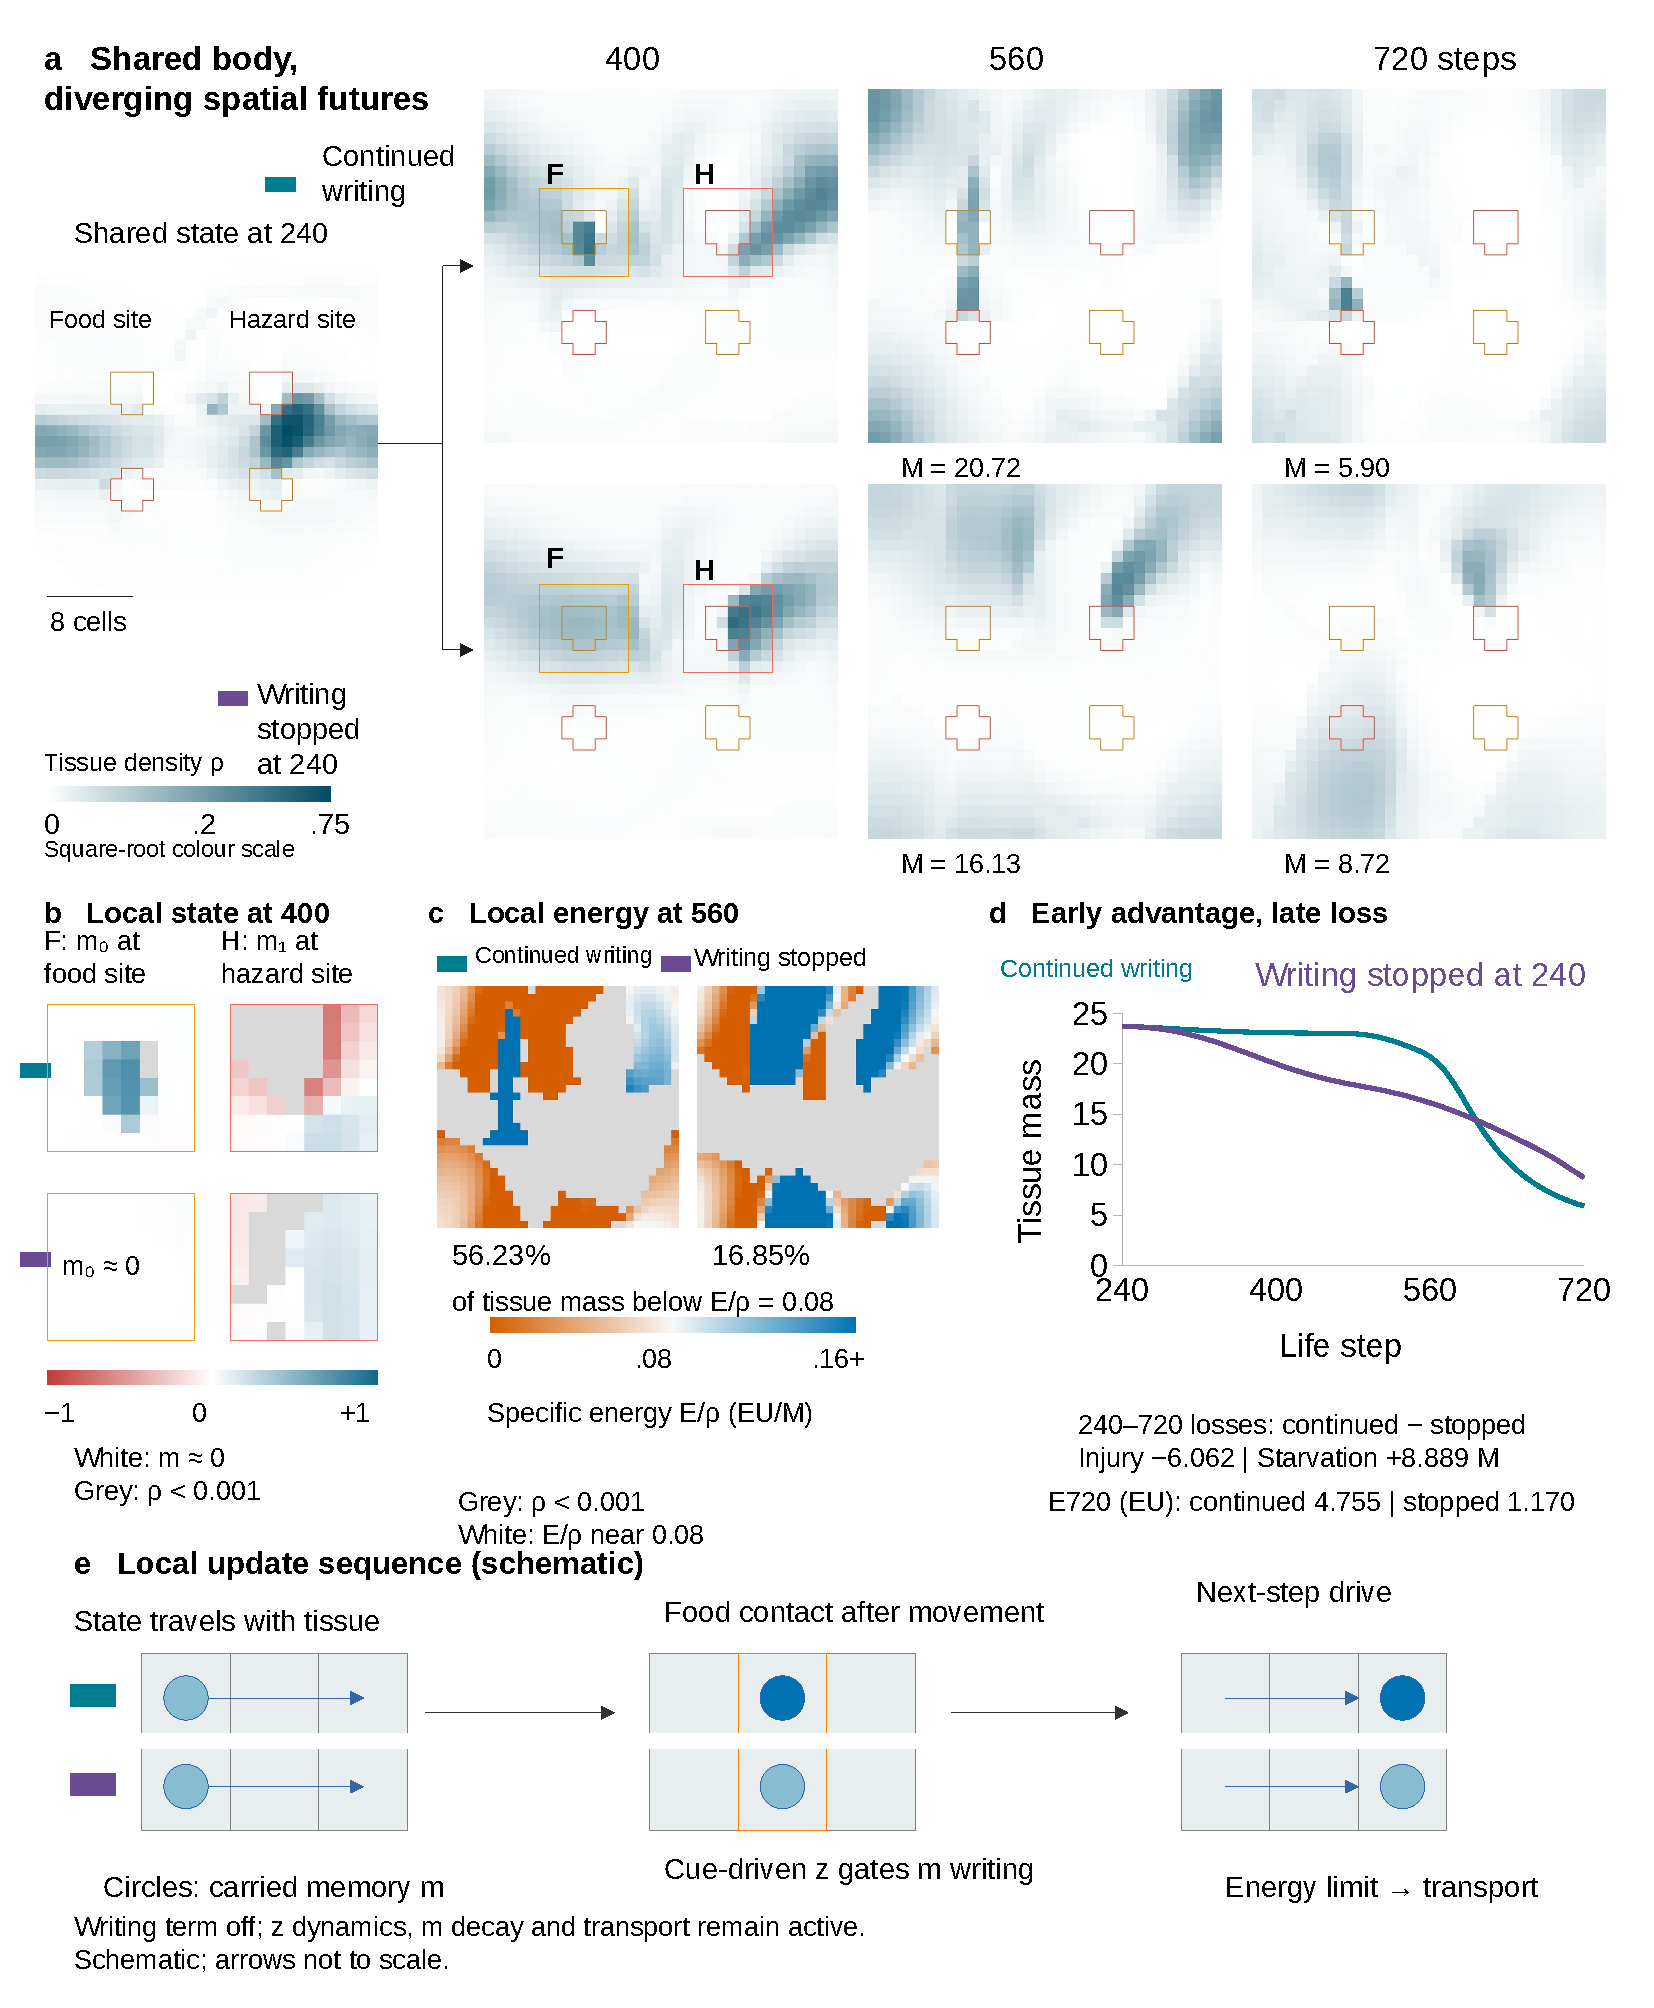
\includegraphics[width=0.90\linewidth]{figures/main/spatial_experience/spatial_state_divergence.pdf}
\caption{\textbf{Shared body, diverging spatial futures.}
\textbf{a,} The same complete acquired body and remaining world at step 240 continue with writing enabled (teal) or new writing stopped (purple). Density scenes at 400, 560 and 720 retain original periodic $32\times32$ coordinates and the same square-root colour scale. F/H mark Food/Hazard sites; F here is a food-site label, not the fuel F of Fig.~\ref{fig:allocation-feedback}. Scale bar, 8 cells.
\textbf{b,c,} Local $m_0/m_1$ at 400 and specific energy at 560 are observed fields, not isolated mediators. Grey masks $\rho<0.001$; low-energy percentages include all tissue mass.
\textbf{d,} The complete 61-point mass path shows early advantage followed by late loss; final energy has the opposite ordering.
\textbf{e,} Schematic of transport, cue-driven eligibility and writing, then subsequent energy-limited movement. Stopping new writing leaves $m$ decay, transport and eligibility active. This model has no tissue birth and is distinct from the generative models; the continued-writing future is reused.}
\label{fig:writing-turnover}
\end{figure}


These observations explain why the spatial process belongs in the main argument. An earlier mass advantage can contain a larger population of poorly fuelled tissue, and different loss mechanisms can reverse a later ordering. The local food- and hazard-associated fields and specific-energy maps reveal where those differences are expressed. They do not identify a unique mediator: local state, energy, shape and subsequent encounters change together after branching. The experiment contains one acquired history and no tissue birth, and its continued-writing future is reused from an existing trajectory. It consequently provides a resolved example of coupled physical consequences, not a population-level estimate of a general learning benefit.

This interpretation is compatible with energetic approaches to active motion\cite{schweitzer,circle,tjhung} and with the broader observation that collective movement depends on distributed interactions\cite{tonertu}. It does not require treating every changing pattern as learning. The evidence is useful because it exposes the actual route from internal-state manipulation to different local resource conditions and loss processes. A successful integrated learner must be evaluated at both levels: the behaviour elicited by experience and the physical trajectory through which that behaviour remains possible.
